\chapter{Human Action Recognition (HAR)}

\begin{quotation}
    \noindent
    \textsf{Across the chapters of these notes we have seen different machine learning models dealing with images (\textit{classification}, \textit{object detection}, \textit{segmentation and instance segmentation} and finally \textit{generative models}); we have seen that also some deep-learning based audio processing techniques can be recasted as an image classification tasks; the \textit{recurrent models} introduced a way to take into account the temporal dependencies among data. In this chapter for the first time, we are approaching to videos and in particular the \textbf{human action recognition tasks (HAR)} whose input is a sequence of images and then a video.
    }
\end{quotation}

\noindent
\section{Introduction, motivations, challenges}
\textbf{Human Action Recognition (HAR)} deals with analyzing a \textbf{video} in order to \textit{identify the human actions} talink place in the video itself, it can be seen as a sort of "video classification".

\begin{figure}[h]
    \centering
    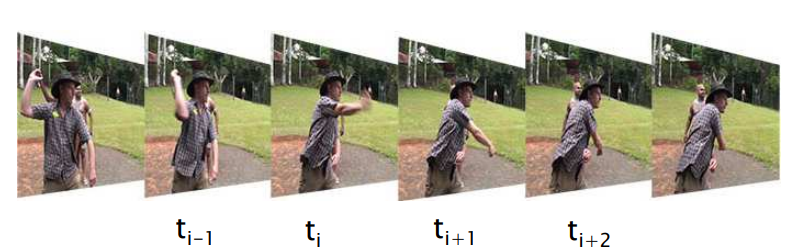
\includegraphics[scale=0.6]{img/video.png}
\end{figure}

\noindent
A video is a 3D signal: $(x,y)$ are the \textit{spatial coordinate} while $t$ is the \textit{temporal coordinate}, fixing the variable $t$ you obtain an image. It is remarkable that new technologies are needed to treat them! An important aspect to be formalized in HAR is the \textbf{time interval} across which the action happens. This can be short (for example an athlete doing squats) or long (a particular action in a football match). \\
We can say that \textbf{Action Recognition} is a computer vision task whose input is a video while the output is the \textit{action label}. Moreover, there different \textit{level of semantics}: action (walking), activity(talking on the phone), event (a birthday part, a soccer game)... where each can be included in the one of an upper semantica level.

We have understood that recognizing human actions is not a trivial task, but \textbf{what is the motivation for doing this?} There are several fields in which such a computer vision task plays an important role: in \textit{robotics} for human-robot interaction and for robot learning, in \textit{smart video-survelillance system} for detecting burglary (anomaly detection), for tagging/summarizing videos an so on. Recognizing actions is useful also for \textit{home monitoring}. \\
We have said that classifying a video is \textbf{challenging}. The following are the main motivations.

\subsection{Challenges in Action Recognition}
\begin{enumerate}
    \itemsep-0.2em
    \item People of which track the acrivity can appear \textbf{at different scales} in different videos; 
    \item In a video scene there could be \textbf{occlusion} in the sense that actions may not be fully visible due to the presence of obstacles in the environment; 
    \item \textbf{Camera movements} are non-negligible in a context where the whole video is analyzed, this can be hand-held (or worn by the subject) or mounted on something which is moving causing the background of the people moving.
    \item It is not said that the video is \textbf{trimmed} to contain only an action and there is no indication of where in the timeline the action occurs.
\end{enumerate}

\subsection{Datasets for action recognition}
Obtaining training datasets for action recognition is extremely challenging, however there are some datasets which provide a quite solid reference point for addressing such taks. The following is a (non-exhaustive) list of well-known datasets: 
\begin{itemize}
    \itemsep-0.2em
    \item \textsc{HDMB51} (Human Motion DB) it is made up 7K clips from 51 action categories (each with 101 samples), they are taken from public repositories like YouTube; 
    \item \textsc{UCF-101} is another commonly used dataset. It has 13k videos from 101 action categories. There are a lot variations of camera  moriton, object scale and appearance... 
    \item \textsc{Sports 1M} It has 1M sports video from youtube with 487 sports label; 
    \item \textsc{ActivityNet} a dataset of 8 hundred hours of video for human activity understanding; 
    \item \textsc{Kinetics-700} it has 700 classes of human-human or human-object \textit{interactions}.
\end{itemize} 

\section{Approaches to action recognition}
There are mainly two approaches for action recognition which differ in the way the features related to the motion are obtained.

\subsection{Hand-crafted approaches}
In this case the feature are \textit{hand-crafted} in the sense that some (non-neural) techniques are used based on the meaning that the motion assumes for sequences of images. The typical structure of any hand-crafted approach for action recognition is the following: 

\begin{figure}[h]
    \centering
    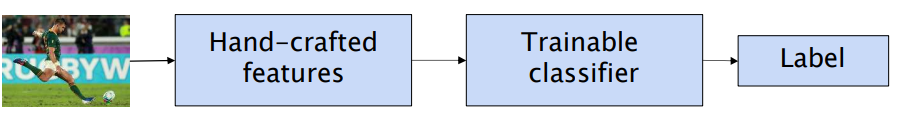
\includegraphics[scale=0.7]{img/handCraft.png}
    \caption{Hand-Crafted approach pipeline}
\end{figure}

The designed features (the first step to carry out) are fed to a trainable classifier which will predict the action represented in that specific video. Now we are going to present some tipologies of hand-features which were widely used for classifying actions before the deep learning advent.

\subsubsection{Motion History Images (MHI)}
Let us think about an action from the point of view of the images, there are \textit{different changes in shapes}. \textbf{Motion History Images} are images in which the \textbf{pixel intensity} is a function of motion at that location. Leveraging on such a representation, some features can be extracted for representing the action. In practice the images represent recent movement with \textbf{brighter intensities} and older movements with a \textbf{dimmer intensity}.

\begin{figure}[h]
    \centering
    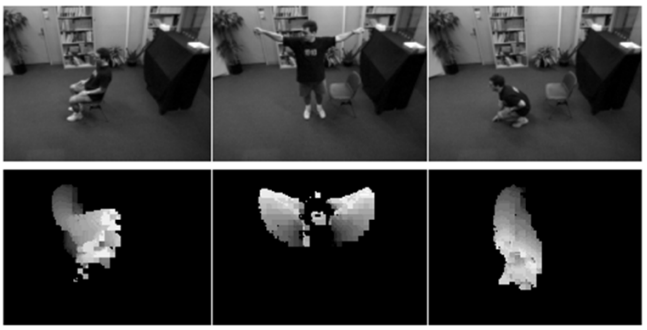
\includegraphics[scale=0.7]{img/MHI.png}
    \caption{Examples of MHIs}
\end{figure}

In this figure you can see the brighter area which are associated to pixels in which the motion is detected, the dimmer areas are associated to motions at previous time instant. The resulting images are gray scale ones in which the intensity at the time $t$ of the pixel in position $(x,y)$is  
\begin{equation*}
    H(x,y,t)=\begin{cases}
        \tau&\text{if motion is detected at } (x,y) \ \text{at time } t\\
        \max(0,H(x,y,t-1)-\Delta{t})&\text{otherwise}
    \end{cases}
\end{equation*}
where $\tau$ is the maximum intensity (usually 255), while $\Delta{t}$ is the decay rate, which decrease the brightness of a certain factor with respect to the previous MHI. At this point is clear that  a new motion history image is retrieved for each pair of frames in the video. This approach is used when there are some conditions, otherwise it will provide you poor quality features for your task! In particular in the case when there is background motion (due to camera movement), flickering light or something related, you are supposed to change the technique.

\subsubsection{Optical flow (general idea)}
This is an highly effective technique for retrieving useful features for representing motion. The underlying idea is that if you focus on a particular pixel at the instant $t$, this pixel will describe a certain \textbf{trajectory} during the video, in particular between one frame and the following can be captured the changes in directions (velocity) of that pixel. The result of this "tracking process" is an image, the \textbf{optical flow image}, in which there is a vector field (each vector related to a pixel). Starting from each vector a color wheel can be used, in particular: \textit{Hue $\to$ Direction} and \textit{Saturation $\to$ Magnitude}.  The following step is taking a group of optical flow images and giving a label corresponding to the action class. A trainable classifier (neural or not) can be used the action recognition task. This is approach is for sure more robust to noise and brightness issues.


\begin{figure}[h]
    \centering
    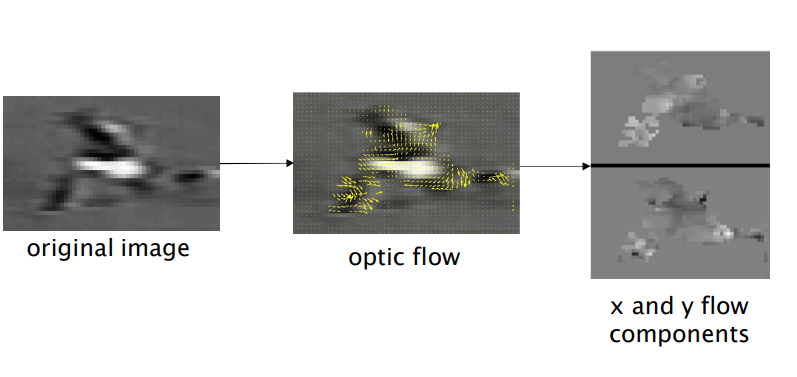
\includegraphics[scale=0.7]{img/optical.png}
    \caption{Optical flow images}
\end{figure}

\subsubsection{Optical flow with Dense trajectories}
We have said that for each pixel image by image we can associate a vector and then combining more images a trajectory. We say that the trajectories coming from the optical flows are \textbf{dense} if the pixels are sampled in a \textit{dense} way at different spatial scales. More details can be found in \cite{dense}, from which is taken the following figure:

\begin{figure}[h]
    \centering
    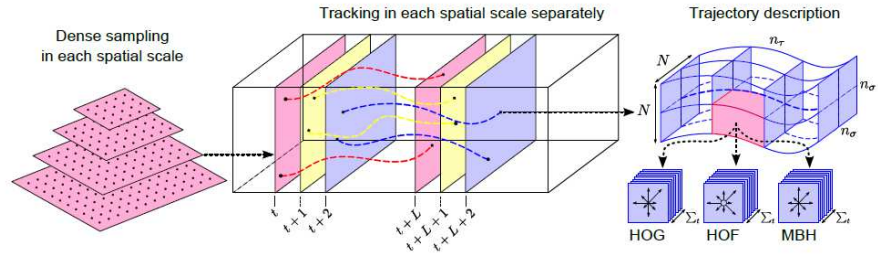
\includegraphics[scale=0.6]{img/densetraj.png}
    \caption{Dense trajectory mechanism} (Different descriptors can be used in order to analyze the volume deriving from $L$-sampling at different spatial scales the video to analyze)
\end{figure}

The tracking is peformed sampling $L$ frames. once for each different scales the tracking has been done, we use some trajectory descriptor to analyze the volume $N\times{N}\times{L}$ deriving from the dense sampling. In the cited paper, the used classifier is an SVM with a $\chi^2$-kernel, however any deep learning techinque can be used.

\subsubsection{Improved dense trajectories}
On a variety of datasets the approach of \textit{dense trajectory} has shown to be a state-of-art approach, however even this approach struggle when camera motions are present. The paper \cite{wang2013action} presents an improvement of the technique used in \cite{dense}.\\
The major improvement is the introduction of a \textbf{separation} between \textbf{foreground} (where objects and human bodies are placed) and \textbf{background} (whose change is  associated with a camera movement). The first step before proceeding in computing the 3D video volume descriptors is \textit{estimate the camera motion} by calculating an \textit{homography between a frame and the following}, at this point the flow vectors related to the camera motion are \underline{ignored} during the computation of the descriptor. Without any doubts, we can say that the \textbf{improved dense trajectories} technique is the state-of-art approach for hand-crafted features in motion analysis.

\begin{figure}[h]
    \centering
    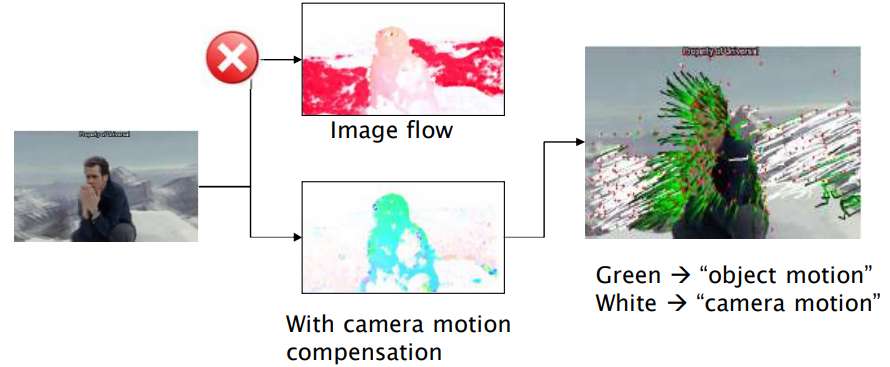
\includegraphics[scale=0.7]{img/improvedense.png}
    \caption{\textbf{Camera compensation in improved dense trajectories} both optical flow and optical flow images are shown. The vectors in white are the ones related to camera motions, for this reason they are ignored.}
\end{figure}

\subsection{Learning-based approaches}
We had the occasion -- in the previous chapter -- to understand that CNNs provide state ot the art \textit{performances} in tasks which involve \textit{analyzing images}. The objective of this section is trying to explain how the standard CNN architectures can be modified in order to process videos and in particular motion information. Here there are two families of architecture: (i) \textsf{Single Stream architecture} they rely on CNN potentiality in order to extract in a trainable way the features from the video frames; (ii) \textsf{Two-streams architecture} in which there are separate streams which analyzes separately the frames singularly and the frames over the time (this is the best approach). The incoming two sections are devoted to the explantation of the main aspects of each model. 

\section{Single-stream architecture}
\begin{figure}[h]
    \centering
    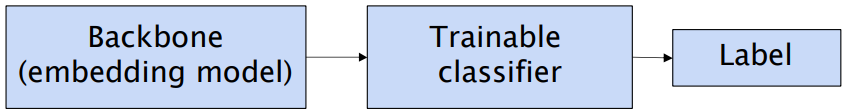
\includegraphics[scale=0.7]{img/SStream.png}
    \caption{Single-stream network}
\end{figure}
The common idea of such an approach is to extract the frame features from a backbone emdedding model, and then \textbf{fuse temporal information} from consecutive frames, where the fusion is not a simple combination of logits. The challenge here is that in a \textbf{single pipeline} there are both spatial and temporal dimensions to manage. The aspect to be discussed are: 
\begin{itemize}
    \itemsep-0.3em
    \item What is an effective way to fuse frames?
    \item How to effectively exploit the temporal dimension?
\end{itemize} 

\subsection{A first approach: Fusing temporal information}
In a standard CNN each frame is processed at a time doing a classification per-image. At the opposite modifying the way the NN takes the input, there mainly \textbf{three ways to fuse} the video frames (see \cite{karpathy2014large}).

\begin{figure}[h]
    \centering
    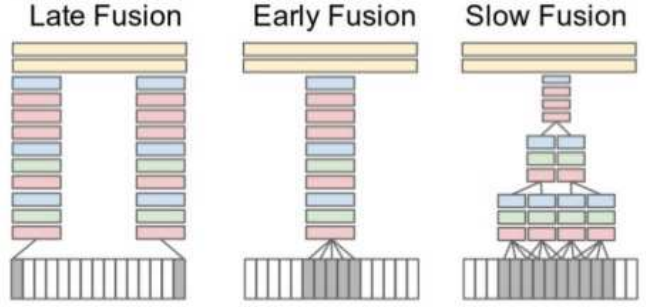
\includegraphics[scale=0.8]{img/Fusion.png}
    \caption{Fusion techniques}
    \label{fig:fusion}
\end{figure}

\subsubsection{Early fusion}
Here the information of a full time-window are combined (10 frames in particular), such frames are stacked and the filter of the first level are modified so that they could operate on a temporal extension of $T=10$ frames. This is the reason why the input is 4-dimensional (RGB+temporal dimension).
\subsubsection{Late fusion}
At the opposite in this case two \textit{separated branches} (sharing the same weights) analyze frames at a fixed distance, the streams are then merged in the first fully connected layer of the network classifier.

\subsubsection{Slow fusion}
This a mix between the previous approaches, since the fusion of temporal and spatial information are \textit{slowly} distributed in the architecture. How can be seen in the \Cref{fig:fusion} the number of braches are halved step by step; the first four braches takes four images (two shared), the merge in the second step occurs, until the last stage is reached where all of the information are fused together.\\

\noindent
The results says that \textit{slow fusion} works better than the other and overall the fusion approaches perform quite better with respect to the single frame predictions. However what is missing here, is an effective way to manage the temporal dimension which is of \textit{paramount importance} in action recognition.\\

\subsection*{Toward better spatio-temporal features}
The next quite intuitive step in order to exploit better the temporal dimension is to use model which are suitable for processing sequences, the idea could be that \textbf{recongnizing an action} is performing the analysis of a sequence of frames. First attempts were based on first extract (separately) the features by using a CNN backbone then pass them to a RNN. Very unsatisfactory resutls were obtained following that direction.

\subsection{\textsf{Long-term Recurrent CNN (LRCNN)}}
In the architecture proposed in \citeauthor{donahue2015long}, \cite{donahue2015long} there is the cascade of a convolutional block (playing the role of encoder) and an LSTM decoder which provides the description of the activity in the video. In the training phase each video is split in 16 clips, whose frames are sampled with a distance of 8 unities. An end-to-end training can be used for the model.
\begin{figure}[h]
    \centering
    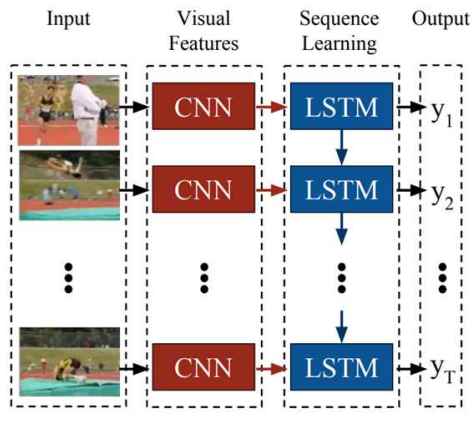
\includegraphics[scale=0.7]{img/LRCNN.png}
    \caption{Long-term Recurrent CNN architecture}
\end{figure}

The fact of splitting the video in clips result in a false label assigment issue since if the real-action has a short duration the label assigned to the clip is not necessarily the correct one. Moreover since LSTM is used as recurrent model, you know that this fails to capture \textbf{long-range temporal information}.

\subsection{\textsf{3D-convolutions}}
In general, any video can be seen as a 4D tensor (RGB+time). Instead of using sequences of images, why not using sequences of clips? This can be done, under the assumption of modifying the convolution process. 2D ConvNets process images producing images and then convolution and pooling are done \textbf{only along the spatial dimension}. In a 3D ConvNet, the processing produces a volume, here convolutions and pooling involve both temporal and spatial dimensions, they are both important in action recognition. The fact of having a third dimension ensure that the temporal information of the input is in some way preserved.

\subsection{\textsf{The C3D architecture}}
C3D (see \citeauthor{c3d}, \cite{c3d}) is a ConvNet which use 3D convolutions to extract features from video volumes input. The kernel is tridimensional here, while using several filters the output is 4-dimensional. 
The architecture of C3D is reported here: 
\begin{figure}[h]
    \centering
    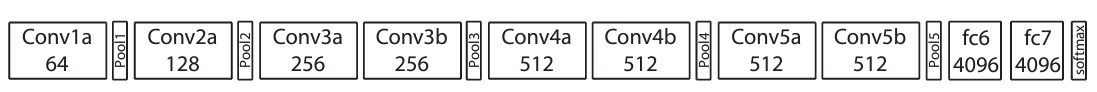
\includegraphics[scale=0.7]{img/c3d.png}
    \caption{C3D architecture}    
\end{figure}
In lower layer always edges and textures are learnt, here in higher layer  we learn more \textbf{complex temporal patterns}. Also in this case there are some limmitations: number of parameters, issues in handling longer temporal dependencies. Again the solution is using combined with the novel C3D model an RNN (tipically LSTM/GRU). Is the idea followed by \citeauthor{montes2016temporal}, \cite{montes2016temporal}. The architecture is shown in the \Cref{fig:c3drnn}

\begin{figure}[h]
    \centering
    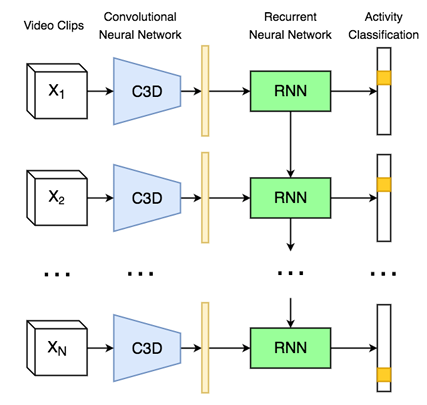
\includegraphics[scale=0.8]{img/c3d+rnn.png}
    \caption{Combining C3D and RNN}
    \label{fig:c3drnn}    
\end{figure}

Given a video, the prediction of the model is a sequence of class probabilities for each 16-frame video clip. The maximum value of the probability (indicated in yellow) is taken as the activity class. Finally only the predicted probability higher than a certain threshold $\gamma$ are kept.

\section{Two-streams architecture}
We have seen that, more or less, the problem which is always present in action recognition is the importance of the temporal dimension and the struggle into embed it in an effective way within the used architecture. The evolution in the field of action recognition led to the paper \textit{\cite{simonyan2014two} \citetitle{simonyan2014two}} by \citeauthor{simonyan2014two} whose architecture is showed in the figure:
\begin{figure}[h]
    \centering
    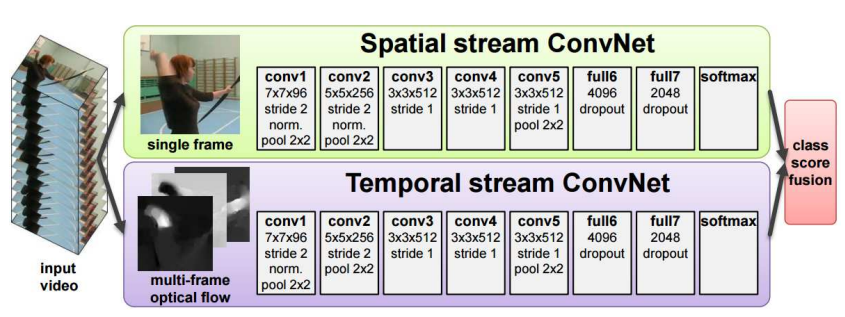
\includegraphics[scale=0.7]{img/2streams.png}
    \caption{Two-streams convolutional network}
    \label{fig:2stream}
\end{figure}
Here there are separated \textbf{temporal} and \textbf{spatial} streams, the first one works with RGB images, while the \textit{temporal branch} is trained using \textbf{multiple optical flow images} which are much more significant than "normal" image in motion analysis\footnote{
    The idea, again, comes  from the human brain and in particular from the structure of the \textit{visual cortex} which is made up two streams: the \underline{ventral strem} (among the other functions) analyze  the objects, while the \underline{dorsal stream} takes care of motion.
}! 
The two streams are trained separately, the final prediction obtained by averaging the predictions across all input frames. The 2-streams architecture, for sure, improves the performances of single stream, however still long-range temporal information are missing, moreover this specific architecture in the \Cref{fig:2stream} cannot be trained end-to-end.

\subsection{3D-fused stream}
Extension of the approach proposed for the 2-stream architecture have been introduced. In particular a 3D ConvNet module takes care of the spatio-temporal analysis (see \cite{carreira2017quo}). This introduce a new 2-stream model inflated with 3D ConvNet (I3D). The novel approaches introduced in the paper are showed in the figure.

\begin{multicols}{2}
    \begin{figure}[H]
        \centering
        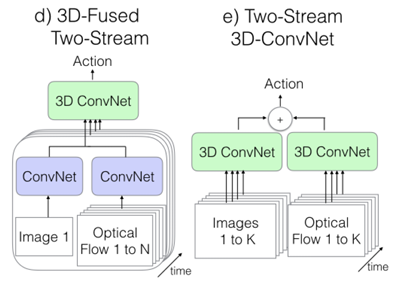
\includegraphics[scale=1]{img/3dfused.png}
    \end{figure}
    In the fisrst case the 3D ConvNet is used to fuse along the time the information coming from the 2-stream network, in the second case (e) the action prediction is performed  by passing the frames of the videos and the optical flow for the frames themselves into two separate 3DConvNets, then the classification is performed by summing the two contributes.\\
    Despite the efforts in improving the existing architecture, \textit{long-range dependencies} still remain a problem!
\end{multicols}

\subsection{Toward good practices: Temporal Segment Network (TSN)}
A possible  solution for solving the long-range dependencies issue is improving the basic two-stream architecture in two ways: 
\begin{enumerate}
    \itemsep-0.3em
    \item Provide a \textbf{sparse sampling} of the input video into \textit{clips} (snippets); 
    \item Implement a \textbf{robust consensus scheme} for aggregating segments predictions.
\end{enumerate}
Such improvements are introduced in \citeauthor{wang2016temporal}, \cite{wang2016temporal} in an architecture called \textbf{Temporal Segment Network (TSN)} and what is gained (among the other things) is that such an architecture is trainable e2e.

\subsubsection{Sparse sampling}
This is \textbf{key operation} which is fundamental here.
TSN architecture operates on a \textit{sequence of short snippets}, obtained by first divinding the video into $K$ segments and then sampling the segment into a \textbf{random small number of frames}. The sampling is \textbf{sparse} since consecutive frames are highly  redundant, a dense sampling of the frames is not needed.

\subsubsection{How TSN operates?}
Each snippet is processed by a two-stream model (as a sequence of RGB frames and stacked optical flows), all models have shared weights. (It is quite obvious that multiple optical flows images are used to span as better as  possible the motion in the selected snippet).

\begin{figure}[h]
    \centering
    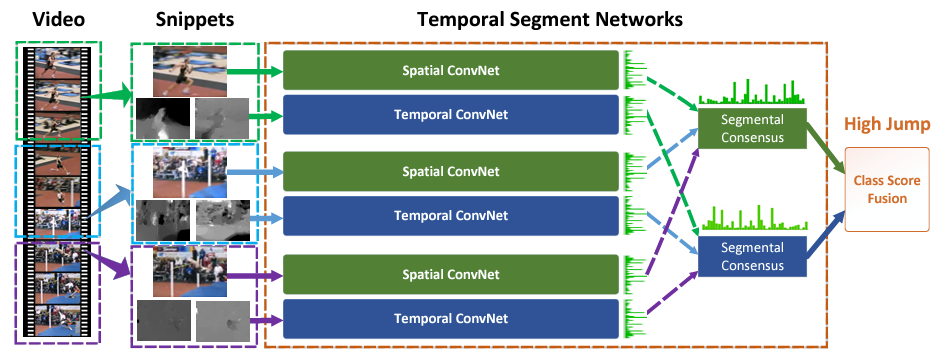
\includegraphics[scale=0.8]{img/TSN.png}
    \caption{\textbf{Temporal segment network}: One input video is divided into K segments and a short snippet is randomly selected from each segment. The class scores of different snippets are fused by an the segmental consensus function to yield segmental consensus, which is a video-level prediction. Predictions from all modalities (temporal and spatial) are then fused to produce the final prediction. ConvNets on all snippets share parameters.}
\end{figure}

The consensus function which is used is not so important, the only important thing is that is a diffeentiable one (also averaging or maximum is good). The scores from different modalities are then fused in a weighted manner to obtain the final prediction. (In the figure the class is \textit{High jump}). In this work other modalities are used like \textit{RGB differences} (describe the appearance change between consecutive frames) and \textit{Warped optical flow} in which the optical flow vector fields are transformed (or "warped") to fit a particular shape or spatial configuration.

\begin{figure}[h]
    \centering
    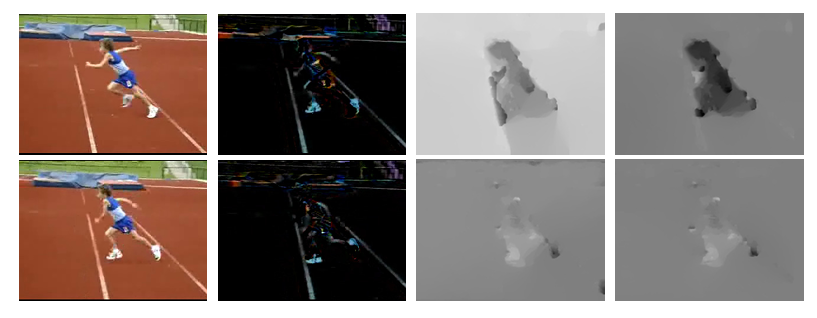
\includegraphics[scale=0.7]{img/4mod.png}
    \caption{Examplex of four different types of input modality:RGB images, RGB differences, optical flow fields (dense), warped optical flow fileds}
\end{figure}

The best result in term of performances is obtained when considering both optical flow and warped optical flow for the temporal stream and RGB images for the spatial flow.